\newcommand{\comment}[1]{}

%\documentclass[a4paper,twocolumn,12pt]{article}

%\documentclass[a4wide,12pt]{report}

%\documentclass[a4wide,12pt]{article}
%\documentclass[informasjonssikkerhet]{gucmasterproject}
\documentclass[informationsecurity]{gucmasterproject}

%\usepackage{pslatex} %% Doesn't seem to work - i.e. convert .eps to .pdf
 
\usepackage[utf8]{inputenc}     % For utf8 encoded .tex files
%\usepackage[latin1]{inputenc}
\usepackage[british]{babel}     % For chapter headings etc.
%\usepackage[pdftex]{graphicx}           % For inclusion of graphics

%From http://math.uib.no/it/tips/
   %% For grafikk
    \usepackage{ifpdf}
    \ifpdf
      \usepackage[pdftex]{graphicx}
      \usepackage{epstopdf}
    \else
      \usepackage[dvips]{graphicx}
    \fi
    %% Her kan du putte dine vanlige pakker og definisjoner



%\usepackage[dvips]{hyperref}    % For cross references in pdf
\usepackage{hyperref}
\usepackage{mdwlist}
\usepackage{url}
\usepackage{float}
\usepackage{todonotes}


\def\UrlFont{\tt}

\begin{document}

\thesistitle{Evading Malicious Code with Concurrent Programming in Parallel Architectures and Their Protection Methods}
\thesisauthor{Caglar SAYIN}
\thesisdate{\gucmasterthesisdate}
\useyear{2013}
\makefrontpages % make the frontpages
%\thesistitlepage % make the ordinary titlepage


\comment{
Front page - including
"   HIG technical report front page including logos etc.
"   The text: "MSc project plan"
"   Title of project
"   Name of author and contact details
"   Date
"   Version

email address
"   MAIS students must include "NISlab" as their affiliation.
Date:22.10.2003

Structure of MSc thesis project plan
Gj�vik University College
}


\chapter*{Revision history}

\begin{center}
\begin{tabular}[H]{|l|p{35em}|}
\hline
Version \#  & Description of change (why, what where - a few sentences)\\
\hline
      0.1   & First version is made available via Fronter\\
\hline
\end{tabular}
\end{center}
\newpage

\begin{abstract}
Abstract (1/2 page)
This document provides format and guidelines  for the 
MSc project descriptions. The document has been produced using MikTeX and TeXnicCenter.

The objective of the abstract is to provide the reader with an understanding of the work to be done and put him in the position to make a 'correct' decision regarding  reading/not reading the report.

The abstract of the project description
{\em must} include
\begin{itemize}
\item a summary of the problem description,
\item motivation and 
\item a summary of the planned contribution from the master project in terms of {\em new} results.
\end{itemize}

\paragraph{Control questions}
\begin{enumerate}
\item Does the abstract have a 'reasonable' length?
\item Is it clear to a non expert (e.g. a typical reader of a newspaper) what problem is addressed?
\item Does a person that has been working in the field find the text informative?
\item Do the results that might be obtained have the potential to be interesting to a lot of people? How interesting to how many and why?
\item Would a decision maker/manager be willing to pay NOK 400.000 to have the project completed (estimated salary costs + overheads) after having read the abstract?  Why/why not?
\end{enumerate}

\end{abstract}


\tableofcontents

\chapter{Introduction (1-2 pages)}
The purpose of introduction chapter is giving the readers blueprint of the subject, the problems that we face, the change in the solutions, as well as motivation of its importance. In addition, It also purpose to form proper research question which will guide thesis. 

\section{Topic covered by the project}
The thesis purposes an architecture of the malware which process parallel, access memory concurrently, conceal itself systematically, shortly that it is likely to be rocket science. However, everything actually started with a simple mathematical theory by John Von Neumann \cite{von1966theory} and the first example of practical malware is writen by Bob Thomas at BBN, and it was called Creeper 

The malware is abbreviation of malicious software. It could be any piece of code which is defined malicious. There is no formal definition of malicious, it could be some software advertise without any contest or it could be self-producing code piece which aim to distribute itself and steal your private information, and it turned an arm race between power holders today.

With development of the first malware, their counter software are created and anti malware software have evolved with them so far. In this race, malware authors are always one step further, because of security's nature. This race between black and white side raised the bar above. The motivation of the information amount and severity influence both today, and that information can be sometimes vital. 


\section{Keywords}
Security, Concurrent Malware Design, Malware, Concurrent, Parallelism and Concurrency

\section{Problem description}
The one of the main and indecipherable problem in security discipline is formulating general threat definition and recognizing malicious activity and all this problems unsurprisingly reflect on information and computer security concept. Security is defined by system’s identification, which involve with purpose, crowd, design structures, network model and so on, and today’s information system which is designed with various architectural forms is protected against malware by general purpose protection tools. In the market, The anti malware tools producers focused on pragmatic solutions to survive, but it leads to that most of these tools are utterly reverse engineering process which works on result instead of reason.

With usual and pragmatic signature based methods, there are two mainstream techniques to detect malicious code which are called static and dynamic analysis.Static analysis identifies malwares mainly with code flow graph and data flow graph on stored file which is not processing. However, On the dynamic side it is a bit more tricky to analyze process, because you are working on the running pieces of codes without knowledge of structures and worse than this, it must concern race condition and memory coherency flaws.

The detection methods and techniques have been adequately worked so far because of the simplicity of architectures and usage of the massive generic computers, However, with increasing of the not standardized, parallel and popular devices like arm’s SoC, it is not hard to estimate their new challenges. It is really likely to evade and obfuscate properly your on-the-fly processes with using uncertain charactership of parallel processing, complexity of concurrent programming, and structure of “Non Uniform Memory Architecture”.


\section{Justification, motivation and benefits}
If malware designing is superficially considered, you could fall in usual fallacy that It is not beneficial and exactly opposite. However, if we can design it, there is always more skillful author who already abuse this vulnerabilities on the black side of the moon. The work we are obligated to actually proof this vulnerabilities and design counter measure against them. In this way, our blessed motivation is finding possible vulnerabilities, and mitigate or eliminate their risk. Otherwise; if we confront with unknown attack, it could be too late to fix and analyze it. For example, some of the most sensational and beneficial papers are criticize malware as same as the thesis (\cite{moser2007limits},\cite{cavallaro2008limits},\cite{egele2012survey}), and their values are undoubted today. 

\section{Research questions}\label{research:questions}

\begin{enumerate}
\item Can a malware model be designed with using parallel and concurrent architecture in order to conceal its presence from detection mechanism?
\item If we can design the mentioned malware, can we build a detection mechanism against these kind of malware's presence?
\item If we build the detection mechanism, What is detection complexity of the algorithms?
\end{enumerate}


\section{Planned contributions}
This Master thesis is looking for better understanding on concurrent malware abilities and their counter-measure. Especially, It will try to show how possible to abuse concurrent memory accessing and how durable recent detection kits. It is quite unique work which we have to consider on the future. Ultimate goal is to eliminate any uncertainties which detection methods encounter with concurrent memory accessing.

\chapter{Related work (3-10 pages)}
This chapter will give an overview of researches about Malware`s self-defense technique, the methods to analyze them, and their application on concurrent architecture. 

\section{Malware Self-Defense}
This section will try to give the literature about malware evasion techniques. This techniques are generally antonym solution which are found by malware authors, however, there are enough surveys about known technique. We classified all these methods in six categories which are code obfuscation, code reuse, anti debugging, anti emulator and visualization and covert channel over network traffic. This taxonomy is well defined by Jonathan A.P Marpaung, et al \cite{marpaung2012survey}, yet malware authors used them to protect their own properties. 


Code obfuscation was originally  found for protecting intellectual property\cite{balakrishnan2005code}, but It aims to puzzle code`s binary against merely static analysis and disassembling\cite{nachenberg1996understanding}. The first known obfuscation method used encryption in order to hide its content. It was called Cascade which is seen first 1986\cite{you2010malware}. This simple architecture of the obfuscation is called packing\cite{internotsecurityteam}. It involve with two part of binary which are slub part, in order to decipher and encipher.\cite{marpaung2012survey}. Cascade was using simple XOR encryption and that was increasing performance.

Early of the 1990s , oligomorphism and polimorphism started to show up\cite{you2010malware}. The main idea behind them is basicly transforming their slub part in each attempt of encryption process\cite{nachenberg1996understanding}. Today, there are two type of  polymorphic approach to generate different variants of slub.\cite{li2011mechanisms}
\begin{itemize}
  \item Rewriting the code each time from pseudo-code so it differs code synthetically which is actually transformation based obfuscation.
  \item Self-cipher itself different, order of these ciphers and using different keys.
\end{itemize}
One of the other important milestone of polymorphic malware is Mutation Engine(MtE) is writen by a Bulgarian virus Author, called The Dark Avanger. It was automated obfuscation tool which actually considered impossible in those times.\cite{anonymous1}

There are also several methods to prevent unpacking process. These methods are collected carefully by Peter Ferrie \cite{ferrie2008anti}. These methods are especially obstacle for automated analysis.

Compare with polymorphic methods, metamorphic approach is more complicated. It is transformation based method instead of encryption  approach.\cite{konstantinou2008metamorphic} Fundamentally, it produce different codes which doing same blue printed semantic. That just mitigate detection possibility because of lack of static code. 

Network traffic, which malware produce are generally Achilles heel for malware, because they are generally adequately unique traffics to be identified\cite{marpaung2012survey}. They usually cover their overt malicious traffic with covert channel methods.\cite{rutkowska2006rootkits}

Code reuse attacks are strong attacks because they do not inject any code in them as obfuscation methods did. They aim to use legitimate software to evade themselves. There are there well known applied version which are return-into-libc, return oriented programming and Frankenstein.

Return into libc attacks were demonstrated by solar designer in 1997 as a method of bypassing non executable stack to executable libc libraries\cite{designer1997getting}. It's object is to change the "ret" infrastructure argument to the known address possibly libc library(stdio, system, etc). However, this attack is limited with libc libraries, which we improved with return oriented programming. 

Return oriented programming is more flex version of retur-into-libc attack, which is introduced by Shacham in 2007\cite{shacham2007geometry}. Return oriented programming purpose a programming language with small gadgets(instruction bound) which involve all ability of Turing's machine\cite{roemer2012return}. Frankenstein is one of the novel application of return oriented programming by Vishwath Mohan and Kevin W. Hamlen\cite{mohan2012frankenstein}.

Anti debugging and anti emulator methods are really usual for today's malware. The survey of Chen Xu et al. showed us in 2008, majority of 6900 on-the-air malware could evade their self with exhibiting benign behavior in sandboxes, debuggers, and virtual machines.\cite{chen2008towards}. VM and debuggers are most important element of dynamic analysis techniques in autonomous sector, because it must run the file just before it touch the working environment. Yet, it is not that knotty to determine whether working environment is virtual or not. Fuzzing cpu bechmarks and comparing results entropy is a good way to determine virtual machines.\cite{franklin2008remote}

Rootkits are the piece of malicious code which aims integrity of the system state.
\section{Malware analysis methods}

\begin{figure}[h]
    \centering
    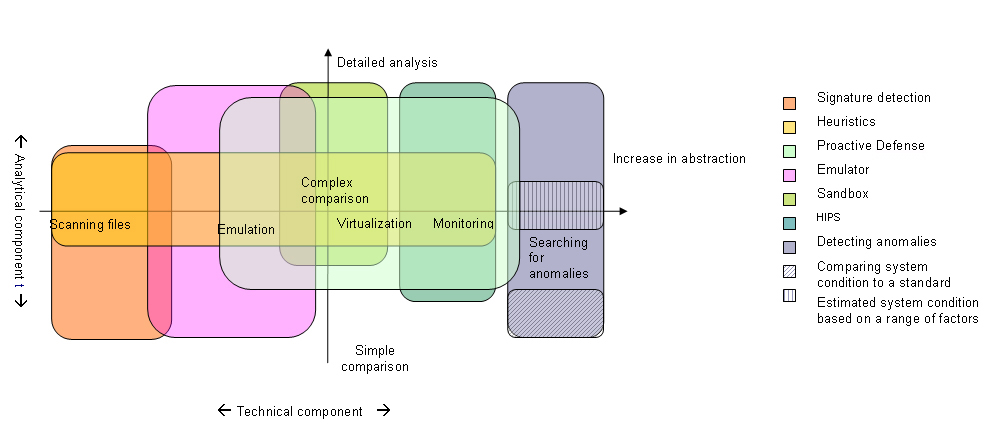
\includegraphics[width=1\textwidth]{alisa_1007_pic1_en.jpg}
    \caption{Detection models \cite{Shevchenko2007detc}}
    \label{fig:awesome_image}
\end{figure}
Malware analysis medhods could be considered two dimensional plane which are "anomaly, signature based detection technique" and "Statistic and dynamic analysis method". 



There are also several applied techniques, which combine terminology above. 
\begin{description}
\item[N-gram] It is a anomaly  based heuristic detection method algorithm. It is a bit costly process and not practical for client side analysis. It could be fit for honey pot analysis \cite{reddy2006n} \cite{abou2004n} \cite{abou2004detection}. They are capable against to zero time malwares and that could makes it futures malware detection system. 
\item[Sequential approach on system and funtion call] This approach is anomaly based dynamic analysis and observing and recording the flow graph of systems and function calls and  try to analysis anomaly behaviors.\cite{kendall2007practical}
\item[Taint] It is also called data flow analysis or data flow graph. It is basic tracking marked data values during execution.\cite{saxena2008efficient}\cite{saxena2008efficient}\cite{smith2007principles}
\item[Control Flow Graph] They are one of the most important arm of commercial autonomous malware detection tools\cite{lee2010detecting} \cite{christodorescu2006static} \cite{christodorescu2005semantics}. After the invention of the polymorphic and metamorphic, syntactic analysis could not bear with them. Then we moved to upper layer of information, semantic layer. Semantic can be representation of code flow, and the routes of the code are adequate to produce signature to identify malware. This methods are a member of static analysis and disassembling and source code analysis job.
\item[Network Monitoring] Malware intention of the communication over network actually big clue to detect them. They generally use unique hostname, ip adress or specific protocol with particular way \cite{marpaung2012survey}.
\end{description}

\chapter{Choice of methods (2-5 pages)}
This section is to include a description of the methods to be used,
including references to literature describing the methods to be used
(e.g. qualitative, quantitative, interviews, surveys,
questionnaire,  model building etc.)
For each of the research questions to be addressed,
the chapter is to explain why the method is
\begin{itemize}
\item appropriate
\item likely to provide the desired knowledge/information.
\end{itemize}

\chapter{Milestones, deliverables and resources (2-5 pages)}
The purpose of this chapter is to convince the reader that you know exactly what to do.
This chapter gives a description of how the project is to be
broken down into smaller parts and activities.
\begin{enumerate}
\item  What is it you have to do in order to obtain the desired knowledge?
\item  What deliverables are to be produced (MSc thesis report, software,...)
\item  When are the various deliverables going to be available?
\end{enumerate}

For each deliverable, identify 4 versions, having an
'increasing' degree of completeness/quality.
Students are strongly recommended to review each others drafts.
For each version of a deliverable explain why and how this version is to
be better/more complete.  E.g. v1.0: my first draft -
chapter text includes 1/2 page summaries only.
v.2.0: Like v1.0, but comments by NN(who? fellow student)
has been incorporated. v3.0:....

This section is to include a preliminary table of contents for the MSc thesis
(only include 2 levels).

For each of the activities identified, specify
\begin{enumerate}
\item  the time you need to complete each activity both calendar time and 'man-hours'.
\item  hours needed by you
\item  things you need to buy (consumables)
\item  equipment, lab space or facilities you need access to
\item  contributions from others (e.g. survey/interview participants) and how much each will have to contribute in terms of resources (probably time)
\end{enumerate}
At the beginning of this section, provide a 2-3 line summary of the
resource requirements.  This is particularly useful if you have broken
down the task into a lot of small tasks.

\chapter{Feasibility study (1/2-3 pages)}



An analysis of why it is likely that the desired
results can be produced within the given time and
resource bounds.  This may include a description of
\begin{itemize}
\item similar projects completed by others and their 'resource consumption',
\item an attempt to answer parts of the research questions
\item the 'difficult' elements of the work and an explanation of why/how these problems can be solved.  
Alternatively you can explain an 'approximate' solution.
\end{itemize}

\chapter{Risk analysis (1/2-2 pages)}
In this project, there five inevitable risks which we can face during development.

\begin{itemize}
\item The thesis is highly dependent on the hardware, and the cost of the hardware constitute risk on its own. Any case of hardware defect leads to comprise obstacle.
\item Hardware dependency is also leads to logistical and time consuming risk which could result with latency on submit time.
\item Firmware codes which we are planning to work on are mostly undocumented. We could discover their usage by proper reverse engineering and fuzzing process when required, however it is obviously manpower.
\item Most important and highlighting risk is there isn't proper research on this particular area. That means there are strongly possibly hidden risks which could cause other mental and physical result.
\item During testing and purification part, Anti-malware tools could come out with unreliable result. To analyze result properly, we may need to inspect mentioned tools with reverse engineering process which could violate proper usage agreement. To mitigate that kind of risks, we could request research agreement from companies.  
\end{itemize}

\chapter{Ethical and legal considerations (1/4-1 page)}
The content of this document could be used in order to malicious purpose, but any matter or information could be misused in the life and ignorance is not known well as a defense strategy. In this purpose, this thesis aims to enlighten security specialist and system developers against recent way of the possible attacks. 

However, in order to act ethical responsibility, we tried to eliminate practice of tools and piece of codes which could leads malicious usage. In any case, there is no doubt that it is critical to discover and publish vulnerabilities which could cause deep impact before malicious people discover and abuse them.

\begin{quote}

"Virus don't harm, ignorance does."\\
- VxHeaven
\end{quote}




\bibliographystyle{gucmasterthesis}
\bibliography{imt4441}



\end{document}

